\section{Задача}

\begin{enumerate}
	\item Задать произвольную матрицу A\([10,10]\) (функция rand)
	\item С помощью функции \([S,J]=eig(A)\) найти собственные числа и собственные вектора матрицы А
	\item Меняем в цикле первое собственное число \(J(1,1)=J(1,1)*10^i, i = 1..15\). Генерируем матрицы с заданным числом обусловленности \(A=S*J*S^{-1}\).
	\item Для каждой из полученных матриц А определяем погрешность определения вектора Х, для чего : задаем вектор Х, вычисляем вектор \(В=А*Х\), выполняем LU разложение \([L,U]=lu(A)\), находим решение системы линейных алгебраических уравнений \(L*U*X_1=B\) : \(Y=L^{-1}*B\); \(X_1=U^{-1}*Y\).
	\item Для каждого из полученных решений находим погрешность \(err(i)=\frac{norm(X-X_1)}{norm(X)}\)
	\item Строим и анализируем график погрешности в логарифмическом масштабе \(plot(log10(err))\).
\end{enumerate}

\newpage

\section{Ход выполнения работы}

В среде MATLAB был написан код, выполняющий поставленные задачи.

\subsection{Программный код для анализа}
\begin{code}
	\inputminted[breaklines=true, xleftmargin=1em, linenos, frame=single, framesep=10pt, fontsize=\footnotesize, firstline=1, lastline=33]{matlab}{listings/luqr.m}
	\caption{Код в среде MATLAB}
\end{code}

\section{Полученные графики}

\begin{figure}[H]
	\begin{center}
		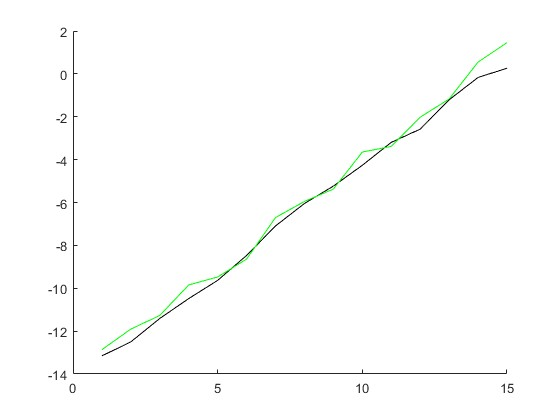
\includegraphics[scale=0.6]{LUQRlog}
		\caption{Графики погрешностей в логарифмическом масштабе. LU - черным, QR - зеленым.}
		\label{pic:luqr} % название для ссылок внутри кода
	\end{center}
\end{figure}

\begin{figure}[H]
	\begin{center}
		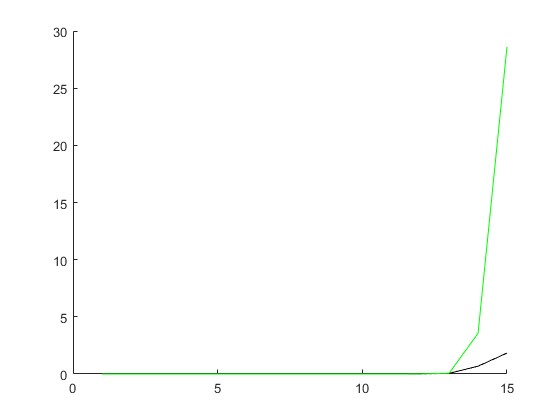
\includegraphics[scale=0.6]{LUQR}
		\caption{Графики погрешностей. LU - черным, QR - зеленым.}
		\label{pic:luqr} % название для ссылок внутри кода
	\end{center}
\end{figure}


\section{Вывод}
Как можно заметить, на более высоких значениях \(i\) (то есть при более высоких значениях числа обусловленности) LU-разложение начинает вести себя более непредсказуемо, чем QR-разложение.